\setchapterpreamble[u]{\margintoc}
\chapter{Grep}
\labch{grep}

We have already seen and used \lstinline|grep| throughout this chapter while discussing regex. \lstinline|grep| is a command that is used to search for patterns in a file. It is used to search for a pattern in a file, and print the lines that match the pattern.

The name \lstinline|grep| comes from the \textbf{g/re/p} command in the \textbf{ed} editor. The \textbf{ed} editor is a line editor, and the \textbf{g/re/p} command is used to search for a pattern in a file, and print the lines that match the pattern. The \lstinline|grep| command is a standalone command that is used to search for a pattern in a file, and print the lines that match the pattern.

\lstinline|grep| can use \textbf{BRE} or \textbf{ERE}, or even \textbf{PCRE} if the \lstinline|-P| flag is used. By default, \lstinline|grep| matches using the \textbf{BRE} engine.

\begin{lstlisting}[language=bash]
$ grep "[aeiou]" -o <<< "hello how are you?"
e
o
o
a
e
o
u
\end{lstlisting}

\section{Regex Engine}

However, \lstinline|grep| can also use the \textbf{ERE} engine using the \lstinline|-E| flag. This is useful when we want to use the special characters like \lstinline|+|, \lstinline|?|, \lstinline|(|, \lstinline|)|, \lstinline|{|, \lstinline|}|, and \lstinline:|: without escaping them.
\sidenote{
 There is also an executable called \lstinline|egrep|, which is the same as \lstinline|grep -E|. It is provided for compatibility with older Unix systems. It is not recommended to use \lstinline|egrep|, as it is deprecated and not present in all systems. You should use \lstinline|grep -E| instead.
}

\begin{lstlisting}[language=bash]
$ grep -E "p+" -o <<< "apple and pineapples"
pp
p
pp
\end{lstlisting}

Sometimes, it is required to not use regex at all, and simply search for a string. We can use the \lstinline|-F| flag to search for a fixed string, and not a regex.
This will search for any line that has the substring. Any symbol that has special meaning in regex will be treated as a literal character.

\begin{lstlisting}[language=bash]
$ grep -F "a+b*c=?" -o <<< "What is a+b*c=?"
a+b*c=?
\end{lstlisting}

This mode is useful if you want to match any arbritary string in a file, and do not know what the string is going to be, thus not allowing you to escape the special characters.

\begin{lstlisting}[language=bash]
$ cat data.txt
Hello, this is a file
with a lot of equations
1. a^2 + b^2 = c^2 for right angle triangles
2. E = mc^2
3. F = ma
4. The meaning of life, the universe, and everything = 42
$ read -r -p "What to search for? " pattern
What to search for? ^2
$ grep "$pattern" data.txt
2. E = mc^2
$ grep -F "$pattern" data.txt
1. a^2 + b^2 = c^2 for right angle triangles
2. E = mc^2
\end{lstlisting}

In the above example, you can see a file full of equations, thus special symbols.
If we want to dynamically input what to search for, we can use the \lstinline|read| command to read the input from the user, and then use \lstinline|grep| to search for the pattern. If we use the \lstinline|-F| flag, we can search for the pattern as a fixed string, and not as a regex.

Here we wanted to find all the quadratic equations, and thus searched for \lstinline|^2|.
However, observe that the \lstinline|grep|, without the \lstinline|-F| flag, did not match the first equation which has multiple \lstinline|^2| in it, because it is treating \lstinline|^| with its special meaning of \textbf{start of line anchor}.

If we were statically providing the search string, we can simply escape the special characters, and use \lstinline|grep| without the \lstinline|-F| flag. But in cases like this, it is easier to simply use the \lstinline|-F| to not use regular expression and simply find substrings.

\section{PCRE}

Similarly, there are situations where the ERE engine is not powerful enough and we need to use the \textbf{PCRE} engine. We can use the \lstinline|-P| flag to use the PCRE engine.

\begin{lstlisting}[language=bash]
$ cat data.txt
Hello, this is a file
with a lot of equations
1. a^2 + b^2 = c^2 for right angle triangles
2. E = mc^2
3. F = ma
4. The meaning of life, the universe, and everything = 42
$ grep -P "c\^2" data.txt
1. a^2 + b^2 = c^2 for right angle triangles
2. E = mc^2
$ grep -P "c\^2(?=.*triangle)" data.txt
1. a^2 + b^2 = c^2 for right angle triangles
\end{lstlisting}

Here, if we want to find all the equations with \lstinline|c^2|, but only if that equation also mentions "triangle" somewhere after the \lstinline|c^2|, then we can use lookahead assertions of PCRE to accomplish that.
Here, the \lstinline|.*| matches any character zero or more times, and the \lstinline|triangle| matches the string "triangle".
Putting it inside a lookahead assertion (\lstinline|(?= )|) ensures that the pattern is present, but not part of the match.

This can be confirmed by using the \lstinline|-o| flag to print only the matched part of the line.

\begin{lstlisting}[language=bash]
$ grep -P "c\^2(?=.*triangle)" -o data.txt
c^2
\end{lstlisting}

\section{Print Only Matching Part}

We have been using the \lstinline|-o| flag extensively to print only the matching part of the line. This is useful when we want to extract only the part of the line that matches the pattern and not the entire line.
This is also very useful for debugging regex, as we can see what part of the line is actually matching the pattern.

If we do not use \lstinline|-o|, then any line having one or more match will be printed entirely, and the matches will be colored red
\sidenote{
  \lstinline|grep| will color the match only if you pass the flag \lstinline|--color=always|, or if the flag is set to \lstinline|--color=auto| and the terminal supports color output. Otherwise no ANSI-escape code is printed by grep.\\ \\
  You can also change the color of the match by setting the \lstinline|GREP_COLORS| environment variable. The default color is red, but you can change it to any color you want.
}
,however, if two consequtive matches are present, it becomes hard to distinguish between the two matches.

If we use the \lstinline|-o| flag, then only the matching part of the line is printed, and each match is printed on a new line, making it easy to see exactly which parts are matched.

\begin{lstlisting}[language=bash]
$ grep -E "o{,3}" <<< "hellooooo"
hellooooo
$ grep -Eo "o{,3}" <<< "hellooooo"
ooo
oo
\end{lstlisting}

In the above example, we ask \lstinline|grep| to match the pattern \lstinline|o{,3}|, that is, match the letter \lstinline|o| zero to three times. If we do not use the \lstinline|-o| flag, then the entire line is printed, and the matches are colored red. This however creates a confusion, even though all the $5$ $o$'s are matched, they cannot obviously be a single match, since a single match can only be of a maximum of $3$ $o$'s. So how are the matches grouped? Is it $3$ $o$'s followed by $1$ $o$ followed by another $o$? Is it $2$ $o$'s followed by $2$ $o$'s followed by one $o$? There seems to be no way to tell from the first output.

However, if we use the \lstinline|-o| flag, then only the matching part of the line is printed, and each match is printed on a new line. It then becomes clear that grep will greedily match as much as possible first, so the first three $o$'s are matched, and then the remaining are grouped as a single match.

\section{Matching Multiple Patterns}

\subsection{Disjunction}

If we want to match multiple patterns, we can use the \lstinline|-e| flag to specify multiple patterns. This is useful when we want to match multiple patterns, and not just a single pattern. Any line containing one or more of the patterns we are searching for will be printed. This is like using an \textbf{OR} clause.

\marginnote{
  In this example, we want to find lines that match the word "file" or the word "life". We can use the \lstinline|-e| flag to specify multiple patterns. The \lstinline|-e| flag is automatically implied if we are searching for a single pattern, however, if we are searching for more than one pattern, we have specify it for all of the patterns, including the first one.
}
\begin{lstlisting}[language=bash]
$ cat data.txt
Hello, this is a file
with a lot of equations
1. a^2 + b^2 = c^2 for right angle triangles
2. E = mc^2
3. F = ma
4. The meaning of life, the universe, and everything = 42
$ grep "file" data.txt
Hello, this is a file
$ grep -e "file" -e "life" data.txt
Hello, this is a file
4. The meaning of life, the universe, and everything = 42
\end{lstlisting}

\subsection{Conjunction}

If we want to match lines that contain all of the patterns we are searching for, we can pipe the output of one \lstinline|grep| to another, to do iterative filtering.

If we want to find lines which start with a number, and also contain the word "a", then we can use two greps to accomplish this.

\marginnote{
  In this example, first we show each of the pattern we are matching, and that they output multiple lines. Then finally we combine both the patterns using pipe to find only the common line in both the outputs. The patterns can be specified in either order. We need to provide the file only in the first grep, and we should \textbf{not} provide a file name to any of the other greps, otherwise it will not use the output of the previous grep as input and just filter from the file instead. \\ \\
  Here the regex \lstinline|^[0-9]| matches any line that starts with a number.
  And the regex \lstinline|\\ba\\b| matches any line that contains the word "a".
  The \lstinline|\\b| is a word boundary, and matches the start or end of a word. Thus it will match the word "a" and not the letter "a" in a word.
}
\begin{lstlisting}[language=bash]
$ cat data.txt
Hello, this is a file
with a lot of equations
1. a^2 + b^2 = c^2 for right angle triangles
2. E = mc^2
3. F = ma
4. The meaning of life, the universe, and everything = 42
$ grep '\ba\b' data.txt
Hello, this is a file
with a lot of equations
1. a^2 + b^2 = c^2 for right angle triangles
$ grep '^[0-9]' data.txt
1. a^2 + b^2 = c^2 for right angle triangles
2. E = mc^2
3. F = ma
4. The meaning of life, the universe, and everything = 42
$ grep '\ba\b' data.txt  | grep '[0-9]'
1. a^2 + b^2 = c^2 for right angle triangles
\end{lstlisting}

\section{Read Patterns from File}

If we have a lot of patterns to search for, we can put them in a file, and use the \lstinline|-f| flag to read the patterns from the file. Each line of the file
is treated as a separate pattern, and any line that matches any of the patterns will be printed.
The type of regex engine used depends on whether \lstinline|-E|, \lstinline|-P|, or \lstinline|-F| is used.

\begin{lstlisting}[language=bash]
$ cat data.txt
p+q=r
apple
e*f=g
$ cat pattern
p+
e*
$ grep -G -f pattern data.txt  -o
p+
e
e
$ grep -F -f pattern data.txt  -o
p+
e*
$ grep -E -f pattern data.txt  -o
p
pp
e
e
\end{lstlisting}

\section{Ignore Case}

If we want to ignore the case of the pattern, we can use the \lstinline|-i| flag. This is useful when we want to match a pattern, but do not care about the case of the pattern, or we are not sure what the case is.

\begin{lstlisting}[language=bash]
$ grep 'apple' /usr/share/dict/words | head
appleberry
appleblossom
applecart
apple-cheeked
appled
appledrane
appledrone
apple-eating
apple-faced
apple-fallow
$ grep -i 'apple' /usr/share/dict/words | head
Apple
appleberry
Appleby
appleblossom
applecart
apple-cheeked
appled
Appledorf
appledrane
appledrone
\end{lstlisting}

As seen above, the first \lstinline|grep| matches only the lines that contain the word "apple", and not "Apple". However, the second \lstinline|grep| matches both "apple" and "Apple".

\section{Invert Match}

Sometimes its easier to specify the patterns we do not want to match, rather than the patterns we want to match. We can use the \lstinline|-v| flag to invert the match, that is, to print only the lines that do not match the pattern.

\begin{lstlisting}[language=bash]
$ cat data.txt
apple
banana
blueberry
blackberry
raspberry
strawberry
$ grep -v 'berry' data.txt
apple
banana
\end{lstlisting}

This is useful when we want to filter out some arbritary stream of data for some patterns.

\marginnote{
  In this example, we are filtering out all the users that have the shell set to \lstinline|nologin|. These are users which cannot be logged into. We can use the \lstinline|-v| flag to invert the match, and print only the users that do not have the shell set to \lstinline|nologin|. Effectively printing all the accounts in the current system that can be logged into.
  \textbf{ntp} uses the \lstinline|/bin/false| shell, which is used to prevent the user from logging in, but is not the same as \lstinline|/usr/bin/nologin|, which is used to prevent the user from logging in and also prints a message to the user.
}
\begin{lstlisting}[language=bash]
$ grep -v 'nologin$' /etc/passwd
root:x:0:0:root:/root:/usr/bin/bash
git:x:971:971:git daemon user:/:/usr/bin/git-shell
ntp:x:87:87:Network Time Protocol:/var/lib/ntp:/bin/false
sayan:x:1000:1001:Sayan:/home/sayan:/bin/bash
test1:x:1001:1002::/home/test1:/usr/bin/bash
\end{lstlisting}

\section{Anchoring}

If we want to match a pattern only at the start of the line, or at the end of the line, we can use the \lstinline|^| and \lstinline|$| anchors respectively.

However, in \lstinline|grep|, if we want to match a pattern that is the entire line, we can use the \lstinline|-x| flag. This is useful when we want to match the entire line, and not just a part of the line.
This is same as wrapping the entire pattern in \lstinline|^$|, but is more readable.

Similarly, if we want to match a pattern that is a word, we can use the \lstinline|-w| flag. This is useful when we want to match a word, and not a part of a word.
This is same as wrapping the entire pattern in \lstinline|\\b|, but is more readable.

\marginnote{
  Observe in this example, if we do not use the \lstinline|-w| flag
  then words that have the substring "apple" will also be matched.
  However, when we use the \lstinline|-w| flag, only the word "apple"
  is matched as a whole word.
}
\begin{lstlisting}[language=bash]
$ grep 'apple' /usr/share/dict/words | tail
stapple
star-apple
strapple
thorn-apple
thrapple
toffee-apple
undappled
ungrapple
ungrappled
ungrappler
$ grep -w 'apple' /usr/share/dict/words | tail
may-apple
oak-apple
pine-apple
pond-apple
rose-apple
snap-apple
sorb-apple
star-apple
thorn-apple
toffee-apple
\end{lstlisting}

\section{Counting Matches}

Sometimes all we want is to see how many lines match the pattern, and not the lines themselves. We can use the \lstinline|-c| flag to count the number of lines that match the pattern.
This is exactly same as piping the output of \lstinline|grep| to \lstinline|wc -l|, but is more readable.

\begin{lstlisting}[language=bash]
$ grep -c 'apple' /usr/share/dict/words
101
$ grep -ic 'apple' /usr/share/dict/words
107
\end{lstlisting}

From this we can quickly see that there are $107-101=6$ lines that
contain the word "Apple" in the file.

We can also print those lines using the \lstinline|diff| command.

\begin{lstlisting}[language=bash]
$ diff <(grep apple /usr/share/dict/words) <(grep -i apple /usr/share/dict/words)
0a1
> Apple
1a3
> Appleby
5a8
> Appledorf
10a14
> Applegate
28a33
> Appleseed
31a37
> Appleton
\end{lstlisting}

Or by using the \lstinline|comm| command.

\begin{marginfigure}
  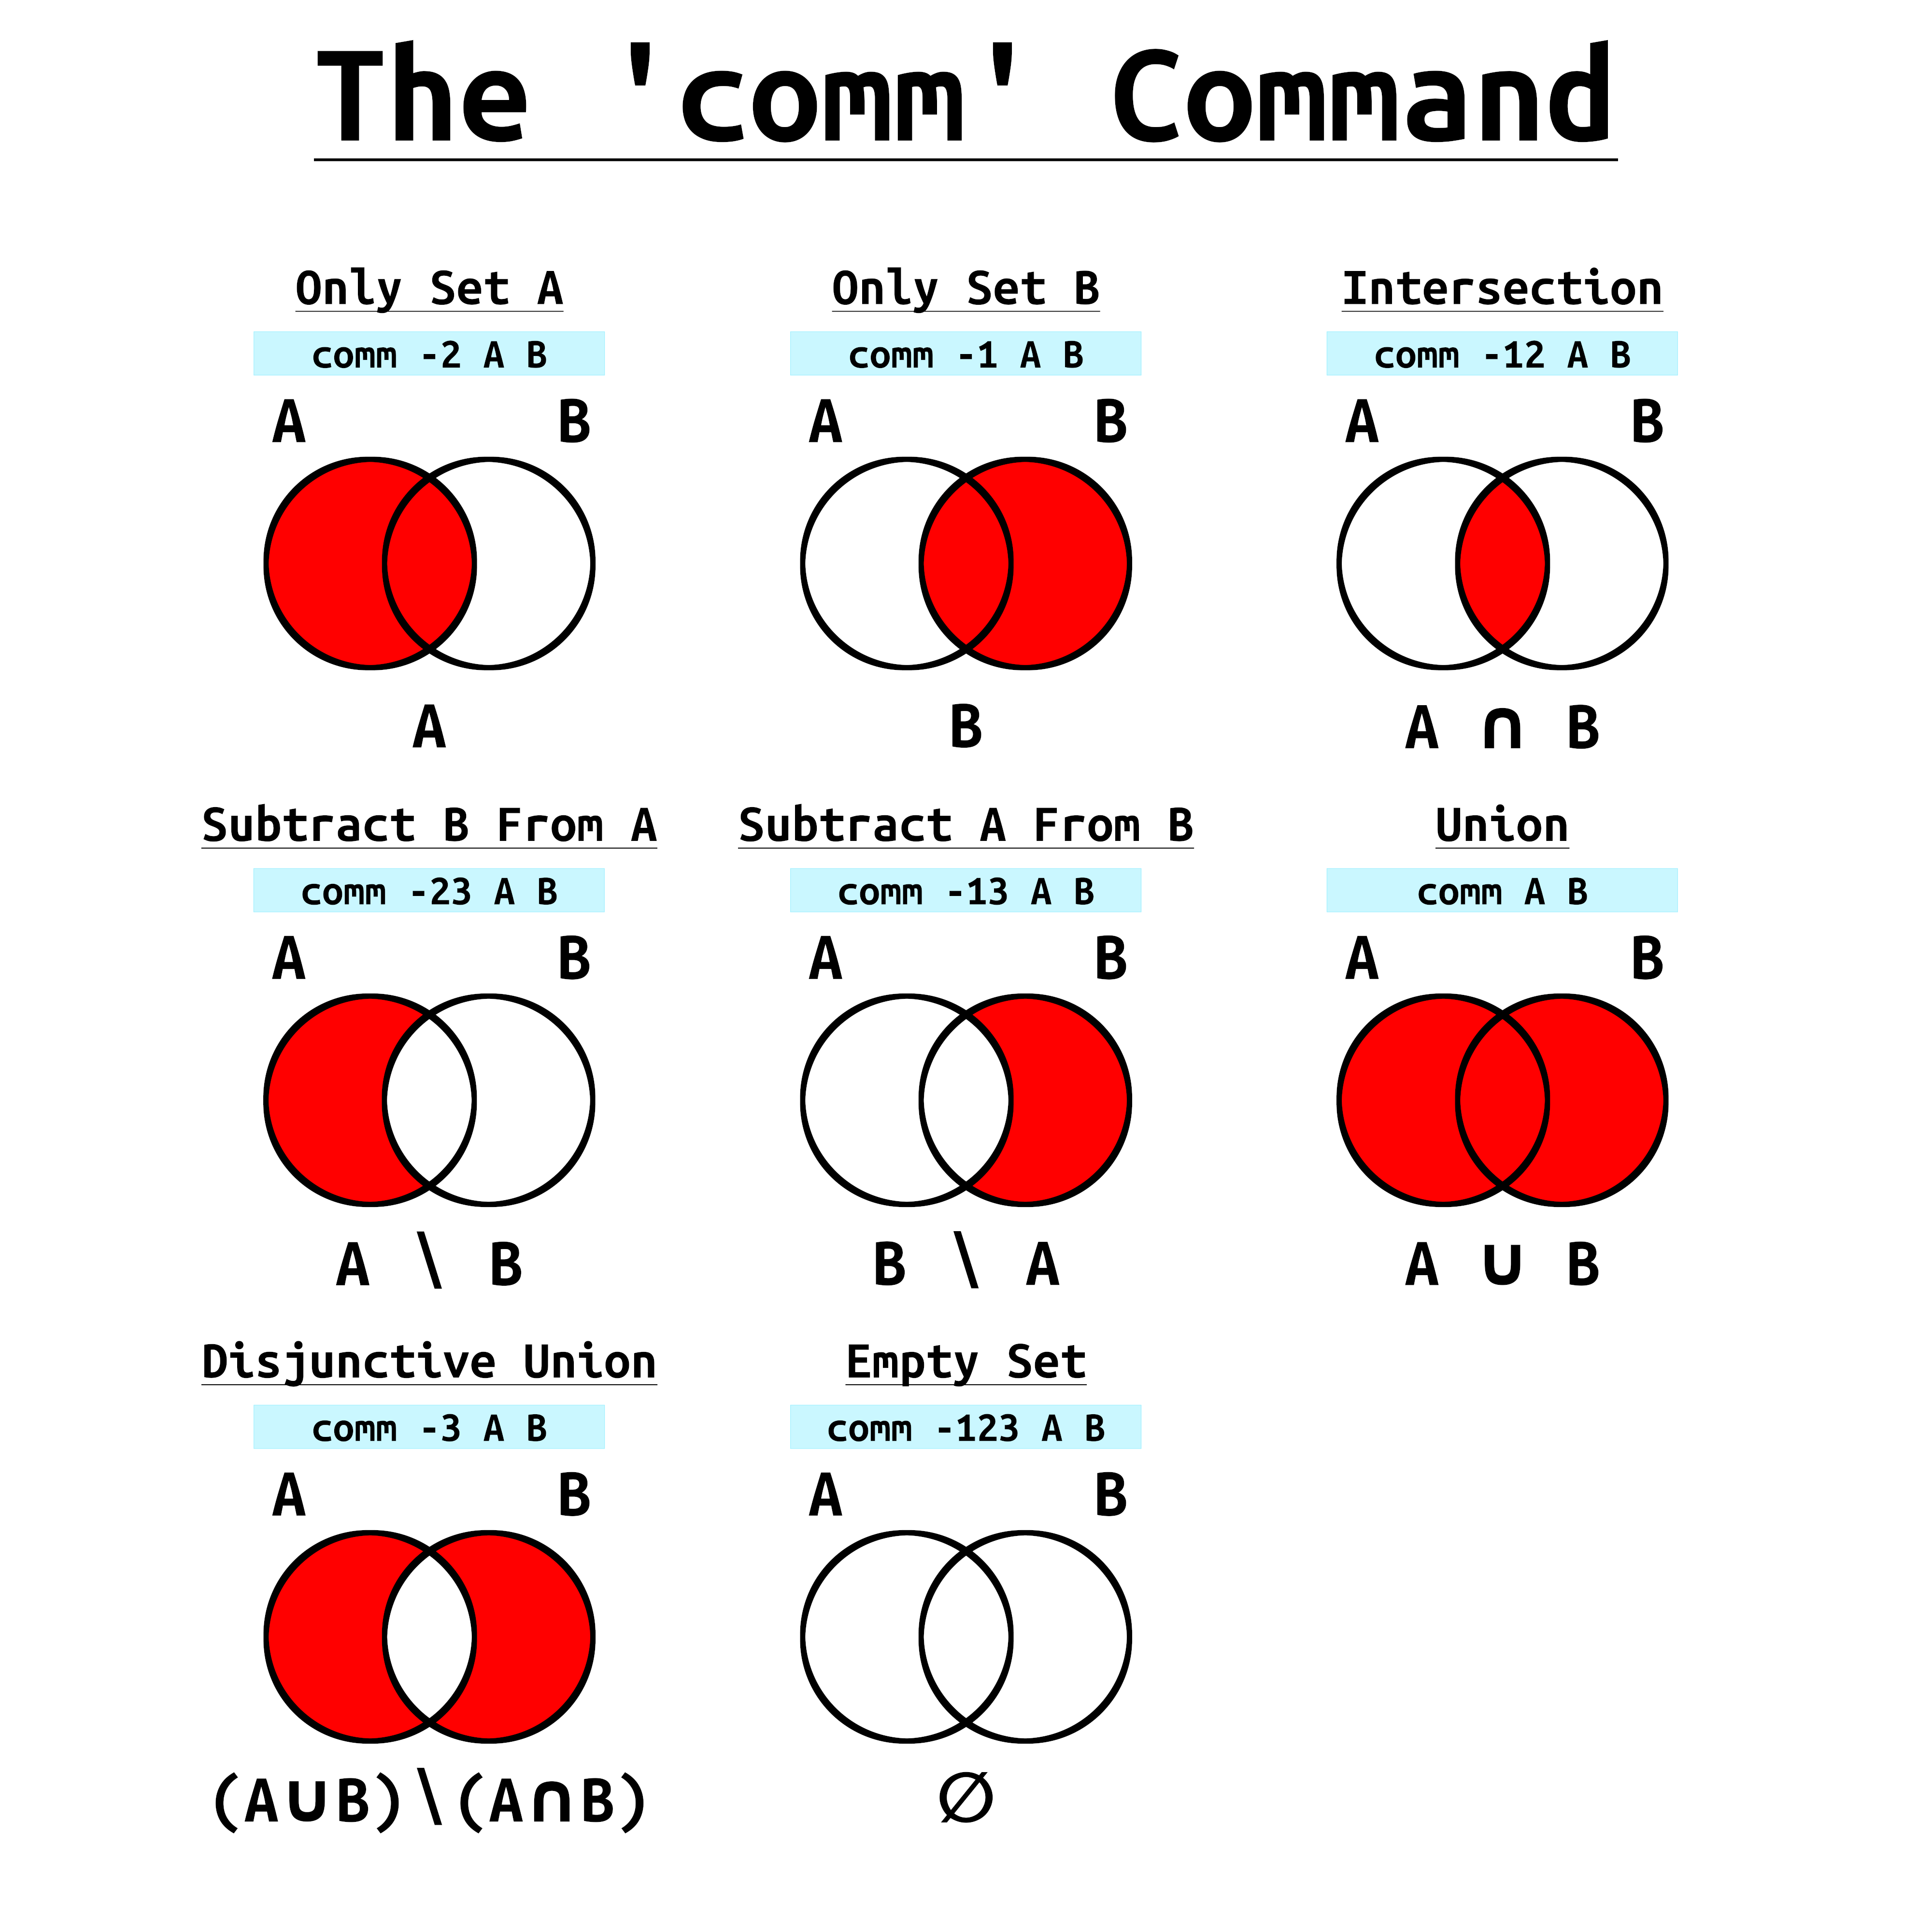
\includegraphics{comm.png}
  \caption{The \lstinline|comm| command}
  \labfig{comm}
\end{marginfigure}

The \lstinline|comm| command is used to compare two sorted files line by line. It is used to find lines that are common, or different between two files. The \lstinline|comm| command requires the input files to be \textbf{sorted}, and it will not work if the files are not sorted. The \lstinline|comm| command has three numbered columns, the first column is the lines that are unique to the first file, the second column is the lines that are unique to the second file, and the third column is the lines that are common to both files. The \lstinline|comm| command is useful when we want to compare two files, and find the differences between them, or find the lines common between them.
\marginnote{
  Observe that we had to sort the files before using \lstinline|comm|, as \lstinline|comm| requires the files to be sorted. We can use the \lstinline|<(command)| syntax to pass the output of a command as a file to another command. This is called process substitution.
}
\begin{lstlisting}[language=bash]
$ comm -13 <(grep apple /usr/share/dict/words | sort) <(grep -i apple /usr/share/dict/words | sort)
Apple
Appleby
Appledorf
Applegate
Appleseed
Appleton
\end{lstlisting}

\section{Print Filename}

Sometimes, we may want to search for a pattern in multiple files, and we want to know which file contains the pattern. We can use the \lstinline|-H| flag to print the filename along with the matched line. This is however the default behaviour in GNU grep if multiple files are passed.

\marginnote{
  In this example, we are passing all the \lstinline|.txt| files in the current directory to \lstinline|grep|, and searching for patterns. The \lstinline|-H| flag is implicit and is used to print the filename along with the matched line. This is useful when we are searching for a pattern in multiple files, and we want to know which file contains the pattern.
}
\begin{lstlisting}[language=bash]
$ cat hello.txt
hello world
hello universe
$ cat linux.txt
this is linux
$ grep hello *txt
hello.txt:hello world
hello.txt:hello universe
$ grep this *txt
linux.txt:this is linux
$ grep i *txt
hello.txt:hello universe
linux.txt:this is linux
\end{lstlisting}

But if we want to suppress the printing of the filename, we can use the \lstinline|-h| flag. This is useful when we are searching for a pattern in multiple files, and we do not want to know which file contains the pattern, just the line.

\begin{lstlisting}[language=bash]
$ cat hello.txt
hello world
hello universe
$ cat linux.txt
this is linux
$ grep -h hello *txt
hello world
hello universe
$ grep -h this *txt
this is linux
$ grep -h i *txt
hello universe
this is linux
\end{lstlisting}

Similarly, if we want to print the filename only if there are multiple files, we can use the \lstinline|-l| flag. This will print \textbf{only} the name of the file that has one or more matches. This mode does not print the filename multiple time even if it has multiple matches on same or different lines.
Thus this is not same as \lstinline/grep pattern files... | cut -d: -f1/.
Rather it is same as \lstinline/grep pattern files... | cut -d: -f1 | uniq/

\section{Limiting Output}

Although we can use \lstinline|head| and \lstinline|tail| to limit the number of lines of output of \lstinline|grep|, \lstinline|grep| also has the \lstinline|-m| flag to limit the number of matches. This is useful when we want to see only the first few matches, and not all the matches.

\marginnote{
  The benefit of using \lstinline|-m| instead of \lstinline|head| is that the output will remain colored if coloring is supported, although it is not visible here, try running both to observe the difference.
}
\begin{lstlisting}[language=bash]
$ grep 'nologin' /etc/passwd
bin:x:1:1::/:/usr/bin/nologin
daemon:x:2:2::/:/usr/bin/nologin
mail:x:8:12::/var/spool/mail:/usr/bin/nologin
ftp:x:14:11::/srv/ftp:/usr/bin/nologin
http:x:33:33::/srv/http:/usr/bin/nologin
nobody:x:65534:65534:Kernel Overflow User:/:/usr/bin/nologin
dbus:x:81:81:System Message Bus:/:/usr/bin/nologin
systemd-coredump:x:984:984:systemd Core Dumper:/:/usr/bin/nologin
systemd-network:x:982:982:systemd Network Management:/:/usr/bin/nologin
systemd-oom:x:981:981:systemd Userspace OOM Killer:/:/usr/bin/nologin
systemd-journal-remote:x:980:980:systemd Journal Remote:/:/usr/bin/nologin
systemd-journal-upload:x:979:979:systemd Journal Upload:/:/usr/bin/nologin
systemd-resolve:x:978:978:systemd Resolver:/:/usr/bin/nologin
systemd-timesync:x:977:977:systemd Time Synchronization:/:/usr/bin/nologin
tss:x:976:976:tss user for tpm2:/:/usr/bin/nologin
uuidd:x:68:68::/:/usr/bin/nologin
avahi:x:974:974:Avahi mDNS/DNS-SD daemon:/:/usr/bin/nologin
named:x:40:40:BIND DNS Server:/:/usr/bin/nologin
dnsmasq:x:973:973:dnsmasq daemon:/:/usr/bin/nologin
geoclue:x:972:972:Geoinformation service:/var/lib/geoclue:/usr/bin/nologin
_talkd:x:970:970:User for legacy talkd server:/:/usr/bin/nologin
nbd:x:969:969:Network Block Device:/var/empty:/usr/bin/nologin
nm-openconnect:x:968:968:NetworkManager OpenConnect:/:/usr/bin/nologin
nm-openvpn:x:967:967:NetworkManager OpenVPN:/:/usr/bin/nologin
nvidia-persistenced:x:143:143:NVIDIA Persistence Daemon:/:/usr/bin/nologin
openvpn:x:965:965:OpenVPN:/:/usr/bin/nologin
partimag:x:110:110:Partimage user:/:/usr/bin/nologin
polkitd:x:102:102:PolicyKit daemon:/:/usr/bin/nologin
rpc:x:32:32:Rpcbind Daemon:/var/lib/rpcbind:/usr/bin/nologin
rpcuser:x:34:34:RPC Service User:/var/lib/nfs:/usr/bin/nologin
rtkit:x:133:133:RealtimeKit:/proc:/usr/bin/nologin
sddm:x:964:964:SDDM Greeter Account:/var/lib/sddm:/usr/bin/nologin
usbmux:x:140:140:usbmux user:/:/usr/bin/nologin
qemu:x:962:962:QEMU user:/:/usr/bin/nologin
cups:x:209:209:cups helper user:/:/usr/bin/nologin
dhcpcd:x:959:959:dhcpcd privilege separation:/:/usr/bin/nologin
redis:x:958:958:Redis in-memory data structure store:/var/lib/redis:/usr/bin/nologin
saned:x:957:957:SANE daemon user:/:/usr/bin/nologin
tor:x:43:43::/var/lib/tor:/usr/bin/nologin
$ grep 'nologin' /etc/passwd | head -n5
bin:x:1:1::/:/usr/bin/nologin
daemon:x:2:2::/:/usr/bin/nologin
mail:x:8:12::/var/spool/mail:/usr/bin/nologin
ftp:x:14:11::/srv/ftp:/usr/bin/nologin
http:x:33:33::/srv/http:/usr/bin/nologin
$ grep 'nologin' /etc/passwd -m5
bin:x:1:1::/:/usr/bin/nologin
daemon:x:2:2::/:/usr/bin/nologin
mail:x:8:12::/var/spool/mail:/usr/bin/nologin
ftp:x:14:11::/srv/ftp:/usr/bin/nologin
http:x:33:33::/srv/http:/usr/bin/nologin
\end{lstlisting}

\begin{lstlisting}[language=bash]
$ cat hello.txt
hello world
hello universe
$ cat linux.txt
this is linux
$ grep -l hello *txt
hello.txt
$ grep -l this *txt
linux.txt
$ grep -l i *txt
hello.txt
linux.txt
\end{lstlisting}

\section{Quiet Quitting}

No, we are not talking about the recent trend of doing the bare minimum in a job.

If we want to suppress the output of \lstinline|grep|, and only see if the pattern was found or not, we can use the \lstinline|-q| flag. This is useful when we want to use \lstinline|grep| in a script, and we do not want to see the output of \lstinline|grep|, just the exit status.
This also implies \lstinline|-m1|, as we can determine the exit status of \lstinline|grep| as soon as we find the first match.

\marginnote{
  In this example we use concepts such as \lstinline|if| and \lstinline|then| to check the exit status of \lstinline|grep|. If the exit status is $0$, then the pattern was found, and we print "world mentioned". If the exit status is $1$, then the pattern was not found, and we do not print anything. \\
  \lstinline|$?| is a special variable that stores the exit status of the last command. If the exit status is $0$, then the command was successful, and if the exit status is $1$, then the command failed. \\
  We will cover these in later chapters.
}
\begin{lstlisting}[language=bash]
$ cat hello.txt
hello world
hello universe
$ grep -q 'world' hello.txt
$ echo $?
0
$ if grep -q 'world' hello.txt ; then echo "world mentioned" ; fi
world mentioned
$ if grep -q 'galaxy' hello.txt ; then echo "galaxy mentioned" ; fi
\end{lstlisting}

\section{Numbering Lines}

If we want to number the lines that match the pattern, we can use the \lstinline|-n| flag. This is useful when we want to see the line number of the lines that match the pattern.

\begin{lstlisting}[language=bash]
$ cat hello.txt
hello world
hello universe
$ grep -n 'hello' hello.txt
1:hello world
2:hello universe
\end{lstlisting}

\section{Recursive Search}

\lstinline|grep| can also search for patterns in directories and subdirectories recursively. We can use the \lstinline|-r| flag to achieve this. This is useful when we want to search for a pattern in multiple files, and we do not know which files contain the pattern, or if the files are nested deeply inside directories.

By default it starts searching from the current directory, but we can specify the directory to start searching from as the second argument.

\begin{lstlisting}[language=bash]
$ mkdir -p path/to/some/deeply/nested/folders/like/this
mkdir: created directory 'path'
mkdir: created directory 'path/to'
mkdir: created directory 'path/to/some'
mkdir: created directory 'path/to/some/deeply'
mkdir: created directory 'path/to/some/deeply/nested'
mkdir: created directory 'path/to/some/deeply/nested/folders'
mkdir: created directory 'path/to/some/deeply/nested/folders/like'
mkdir: created directory 'path/to/some/deeply/nested/folders/like/this'
$ echo hello > path/to/some/deeply/nested/folders/like/this/hello.txt
$ echo "hello world" > path/world.txt
$ grep -r hello
path/world.txt:hello world
path/to/some/deeply/nested/folders/like/this/hello.txt:hello
$ grep -r hello path/to/
path/to/some/deeply/nested/folders/like/this/hello.txt:hello
\end{lstlisting}

\section{Context Line Control}

Sometimes it is useful to see a few lines before or after the actual line that
contains the matched pattern. We can use the \lstinline|-A|, \lstinline|-B|, and \lstinline|-C| flags to control the number of lines to print after, before, and around the matched line respectively.
\sidenote{
  The \lstinline|-A| flag is for printing lines \textbf{after} the match, the \lstinline|-B| flag is for printing lines \textbf{before} the match, and the \lstinline|-C| flag is for printing lines both \textbf{before} and \textbf{after} the match.
}

\begin{lstlisting}[language=bash]
$ grep -n sayan /etc/passwd
37:sayan:x:1000:1001:Sayan:/home/sayan:/bin/bash
$ grep -n sayan /etc/passwd -A2
37:sayan:x:1000:1001:Sayan:/home/sayan:/bin/bash
38-qemu:x:962:962:QEMU user:/:/usr/bin/nologin
39-cups:x:209:209:cups helper user:/:/usr/bin/nologin
$ grep -n sayan /etc/passwd -B2
35-sddm:x:964:964:SDDM Greeter Account:/var/lib/sddm:/usr/bin/nologin
36-usbmux:x:140:140:usbmux user:/:/usr/bin/nologin
37:sayan:x:1000:1001:Sayan:/home/sayan:/bin/bash
$ grep -n sayan /etc/passwd -C2
35-sddm:x:964:964:SDDM Greeter Account:/var/lib/sddm:/usr/bin/nologin
36-usbmux:x:140:140:usbmux user:/:/usr/bin/nologin
37:sayan:x:1000:1001:Sayan:/home/sayan:/bin/bash
38-qemu:x:962:962:QEMU user:/:/usr/bin/nologin
39-cups:x:209:209:cups helper user:/:/usr/bin/nologin
\end{lstlisting}

These were some of the flags that can be used with \lstinline|grep| to control the output. There are many more flags that can be used with \lstinline|grep|, and you can see them by running \lstinline|man grep|.

Now that we have learnt some of the flags on their own, let us try to accomplish certain tasks using multiple flags together.

\section{Finding Lines Common in Two Files}

If we have two files which has some lines of text, and our job is to find
the lines that are common in both, we can use \lstinline|comm| if the files
are sorted, or we can sort the files before passing it to \lstinline|comm| if we are allowed to have the output sorted.

But if we are not allowed to sort the files, we can use \lstinline|grep| to accomplish this.

\begin{lstlisting}[language=bash]
$ cat file1.txt
this is file1
this.*
a common line
is to check if it misinteprets regex
apple
$ cat file2.txt
this is file2
this.*
a common line
is to check if we are checking fixed strings
pineapple
\end{lstlisting}

Ideally the lines that should be detected as being common are the lines

\begin{lstlisting}
this.*
a common line
\end{lstlisting}

Remember that grep allows using a file as the pattern, and it will match any line that matches any of the patterns in the file.
Let us try to use it to provide one file as a pattern, and the other file as the input.

\begin{lstlisting}[language=bash]
$ grep -f file2.txt file1.txt
this is file1
this.*
a common line
\end{lstlisting}

Observe that it is also matching the line \lstinline|this is file1|, which is not common in both the files. This is because the \lstinline|.*| in the pattern \lstinline|this.*| is being interpreted as a regex, and not as a literal character. We can use the \lstinline|-F| flag to treat the pattern as a fixed string, and not as a regex.

\begin{lstlisting}[language=bash]
$ grep -Ff file2.txt file1.txt
this.*
a common line
\end{lstlisting}

So is that it? It looks like we are getting the correct output.
Not yet. If we reverse the order of files, we see that we are not getting the correct output.

\begin{lstlisting}[language=bash]
$ grep -Ff file1.txt file2.txt
this.*
a common line
pineapple
\end{lstlisting}

This is because the \lstinline|apple| in \lstinline|file1.txt| is matching the word \lstinline|pineapple| in \lstinline|file2.txt| as a substring.

If we want to print only lines that match the entire line, we can use the \lstinline|-x| flag.

\begin{lstlisting}[language=bash]
$  grep -Fxf file1.txt file2.txt
this.*
a common line
\end{lstlisting}

Now we are getting the correct output, in the original file order.

If we were to use \lstinline|comm|, we would have to sort the files first, and then use \lstinline|comm| to find the common lines.

\begin{lstlisting}[language=bash]
$ comm -12 file1.txt  file2.txt
comm: file 1 is not in sorted order
comm: file 2 is not in sorted order
comm: input is not in sorted order
$ comm -12 <( sort file1.txt)  <(sort file2.txt)
a common line
this.*
\end{lstlisting}

Observe how the order of output is different.

The trick to mastering grep is to understand the flags, and how they can be combined to accomplish the task at hand. The more you practice, the more you will understand how to use grep effectively. Refer to the practice questions in the VM.

